\section{Specifications of Robot Arm}
\label{sec:spec}

We need to verify robot details before start of working, because in laboratory we have LR Mate 200iB and in RobWork we have LR Mate200iC model. We need make sure is the model of RobWork fit to simulate real robot in the laboratory. Model in RobWork (LR Mate200iC) is depicted in the figure bellow – left and model in laboratory (LR Mate200iB) is depicted bellow – right. As we see from the figure construction from some of the points they are different however in other case similar.

\begin{figure}[H]
  \centering
  \includegraphics[scale= 0.8]{source/fanucModelPhoto.png}
  \caption{Fanuc Models, left: LR Mate 200iC, right: LR Mate 200iB}
  \label{fig:FanucModels}
\end{figure}

\begin{figure}[H]
  \centering
  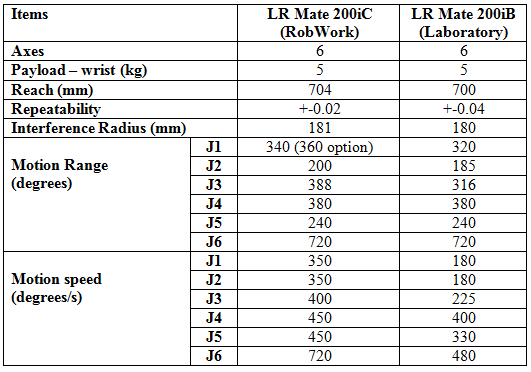
\includegraphics[scale= 0.8]{source/table1.png}
  \caption{Specifications of LR Mate 200iB and LR Mate 200iC}
  \label{fig:tableSpecifications}
\end{figure}

Find the similarities and differences points from which aspects we analyze them. One of the point we chosen specifications of two models, of course this point is not primary. As we see main point here is axes – both models has same number of axes. According this we can say models are similar. Other points from the table are not so important for use – it is payload, reach or motion speed, because they more related to efficiency.

\subsection{Dimensions of the two Models}
Here we try to verify details from dimension aspect. We try find is these models similar in dimensions or not. For instance like one model can be 3 meters high and another 30 centimeters, so they are totally different.  Both models depicted below in the figure 3. Models are quite the same because they both have six revolute axes (we defined in previous chapter). We can try regarding dimension of two models constructing DH parameters and then comparing them.

\begin{figure}[H]
  \centering
  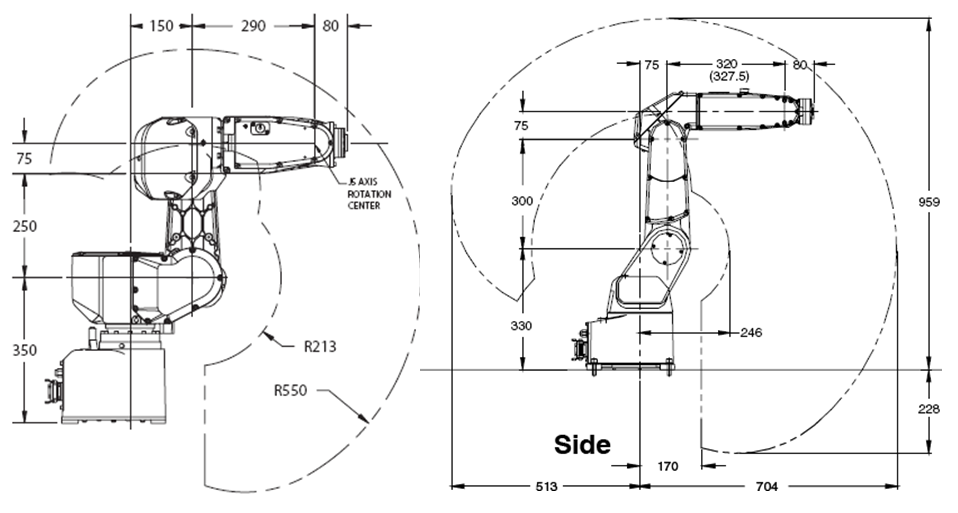
\includegraphics[scale= 0.45]{source/ModelsDimensions.png}
  \caption{left: LR Mate 200iB (Laboratory), right: LR Mate 200iC (RobWork)}
  \label{fig:ModelsDimensions}
\end{figure}

To construct DH parameters, before we need to know what the meanings of the parameters, they defined bellow:

% math 

To construct the DH parameters we need to know the dimensions of both the models, they are shown in the figure 2. At the left LR Mate 200iB model which we use in the laboratory and on the right LR Mate 200iC model which we use only to simulate. Constructed parameters shown in the table 2. 

\begin{figure}[H]
  \centering
  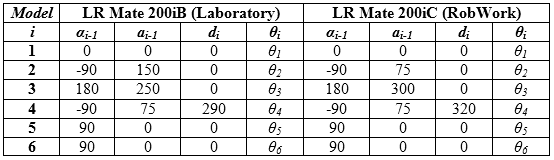
\includegraphics[scale= 0.8]{source/table2.png}
  \caption{DH parameters of LR Mate 200iB and LR Mate 200iC}
  \label{fig:tableParameters}
\end{figure}

From the table 2 we can see that the real model and model which will be used for simulations is quite similar, however some links [1] are different and it makes not the same. However differences not very huge so we make decision that model for simulation can be used as simulator. We have define that LR Mate 200iB will be constructed by defining frames and model LR Mate 200iC is just defining the shapes of 3D model. So we make guarantee that the next part will be simulate real robot model and we only see model in RobWork (LR Mate 200iC), which a little bit different from real model (LR Mate 200iB).

\subsection{Construction of the Cage}
After verification of the details we can measure the dimensions of where the robot stands. LR Mate 200iB stands in the cage as shown in the figure 3 (here is LR Mate 200iC model, because we not make a photo to do better illustrations). Dimensions of the cage measured and depicted by the RobWork, using the xml file were created cage. Robot hand stands on the table and around the robot hand is a cage which guarantees the safety. Position of the LR Mate 200iB on the cage is on the left – up corner (if we look from the front view).

\begin{figure}[H]
  \centering
  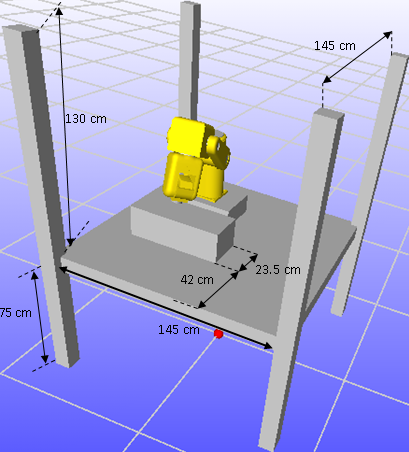
\includegraphics[scale= 0.7]{source/robworkCage.png}
  \caption{Front view of the LR Mate 200i}
  \label{fig:robworkCage}
\end{figure}

Figure 4 shows the robot position from top view and dimensions of the cage where LR Mate 200i stands. As we see shape of the table is square, real table width is a little bit bigger. We use smaller reason to guarantee what we would not damage the cage. Defined smaller work space it will guarantee safety.\newline

Lengths were measured by using the 50 cm ruler. Of course we would like to find the bigger one, so probably of that our measurements have bigger errors and we can imagine that they could be maybe ± 2.5 cm. We do not guarantee that all values precise enough.

\begin{figure}[H]
  \centering
  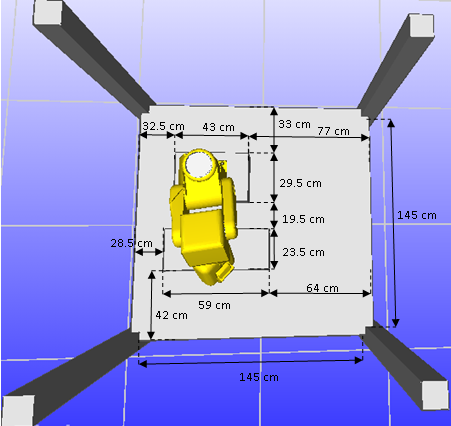
\includegraphics[scale= 0.7]{source/robworkCageDimensions.png}
  \caption{Top view of the LR Mate 200i}
  \label{fig:robworkCageDimensions}
\end{figure}

Regarding this we can set right max theta angles. They will limit movements of the joints. If we do not do this we risk damaging the cage if the errors occur.

\subsection{Construction of Joint Angles}
Joint angles we mean interval of turn between min and max. By default values were set as shown in the figure 5, however we need to change them to guarantee what the robot hand did not move too much. If we allow all these values when everything also will be alright but if the robot fails for some of the reasons than could be a risk to damage the window or even worse injure people around. So that is why we decided to limit turning angle of the robot. 

\begin{figure}[H]
  \centering
  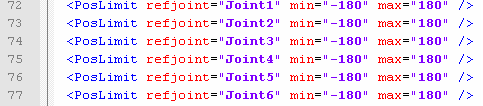
\includegraphics[scale= 0.8]{source/angleDefaultXML.png}
  \caption{Description of LR Mate 200i in Xml (by default)}
  \label{fig:angleDefaultXML}
\end{figure}

Before start we need to illustrate the robot position in the cage and show all measured dimensions. Regarding robot dimensions and joint positions we can start modeling angles of turnings. In the xml file each joint has min and max we set it by $\theta _{min}$ and $\theta _{max}$ here theta is angle limits of turn.

\begin{figure}[H]
  \centering
  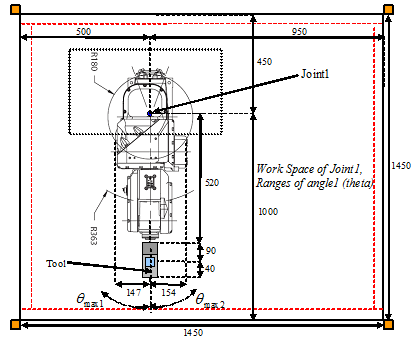
\includegraphics[scale= 1]{source/JointWorkspaceDimensions.png}
  \caption{Work space of Joint1 (Top View)}
  \label{fig:JointWorkspaceDimensions}
\end{figure}

According figure 6 we can calculate max movements of the joint1 or angles: \\

\noindent$\theta _{min}=\theta _{max1}\\
\theta _{max}=\theta _{max2}$

\begin{align}
\theta _{max1}=arctan\left ( \frac{500-x}{520+90+40} \right ) \label{eq:eq0}\\
\theta _{max2}=\frac{\pi }{2}+arctan\left ( \frac{500-x}{520+90+40} \right )\label{eq:eq1}
\end{align}

In the formula 1 value x is error. Depending on the shape of the robot we use x > 154, let us say x = 180. Than we can calculate max movement ranges of the joint 1:

\noindent$\theta _{max1}=arctan\left ( \frac{500-180}{520+90+40} \right )=arctan\left ( \frac{320}{650} \right )\approx 26deg \\
\theta _{max1}=\frac{\pi }{2}+arctan\left ( \frac{500-180}{520+90+40} \right )=\frac{\pi }{2}+arctan\left ( \frac{320}{650} \right )\approx 116deg$\\


We can illustrate angles of theta from another view (view from left). Regarding formula 1 we can also calculate other angles, however we can not do all of them, because joints are dependent each other and we only modeling here statically. 

\begin{figure}[H]
  \centering
  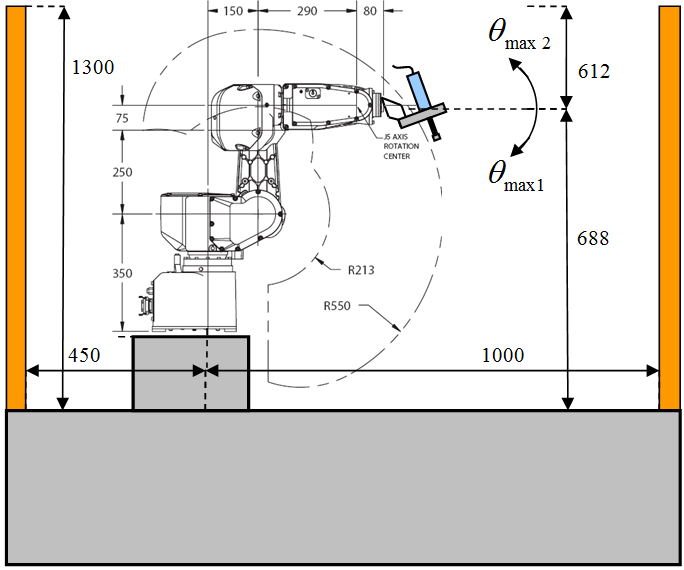
\includegraphics[scale= 0.6]{source/JointWorkspace.png}
  \caption{Work space (Left View)}
  \label{fig:JointWorkspace}
\end{figure}

Our chosen – calculated angles are shown in the figure 8. As we can see angles are much more less than it can be, because of the safety. 

\begin{figure}[H]
  \centering
  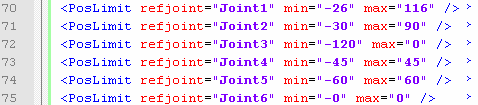
\includegraphics[scale= 0.8]{source/angleXML.png}
  \caption{Description of LR Mate 200i in Xml}
  \label{fig:angleXML}
\end{figure}

\subsection {Modeling the Tool Frame}

Requirement was to have few parameters which let us easily calibrate the tool frame (drill frame). Before that we need to measure the drill which shown in the figure 9 (not very nice). As we see from the figure 9, there are two unknowns a and b. Values of a and b let define the position of the drill. As we see than we changing b than we can shift to right or left and it depends mostly of the drill construction. Second one called a is height control of the drill and it possibly changed many times. For instance if we broken the drill or changed the new one. 

\begin{figure}[H]
  \centering
  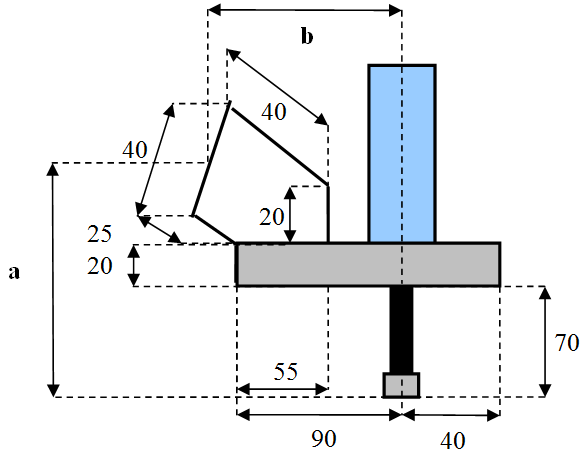
\includegraphics[scale= 0.6]{source/drillDimensions.png}
  \caption{Dimensions of the drill (Tool)}
  \label{fig:drillDimensions}
\end{figure}

Setting of the tool frame were done throw intermediate tool frame. Intermediate tool frame rotate frame by 45 deg, because of the drill construction.  Then we can easily calibrate tool frame according the created intermediate frame. As shown in the figure 10. There are two values a and b (for more details look at the figure 9) value b is width of where drill stand and value a is deep of the drill.

\begin{figure}[H]
  \centering
  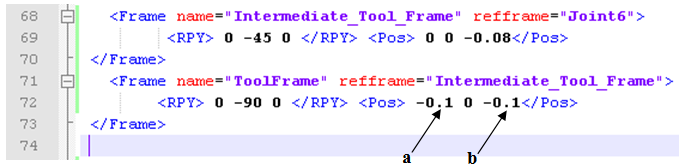
\includegraphics[scale= 0.6]{source/toolCalibrationXML.png}
  \caption{Dimensions of the drill (Tool)}
  \label{fig:toolCalibrationXML}
\end{figure}

Result of the intermediate and tool frames shown in the figure 11. Configuration of it shown in the xml file extract (figure 10). Regarding this we can easily adopt any desired tool. For instance if we get longer drill or different dimensions of tool than we can easily modify xml file and work.

\begin{figure}[H]
  \centering
  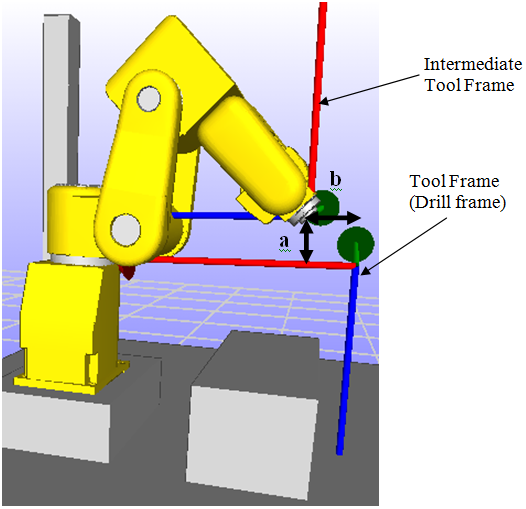
\includegraphics[scale= 0.6]{source/toolFrame.png}
  \caption{Tool frame (drill frame)}
  \label{fig:toolFrame}
\end{figure}

As we can see from the figure 11 tool frame can be easily modified. Tool frame is important for the future parts, like path planner. Path planner takes Cartesian coordinates from the letter model and moves tool frame regarding it. By moving tool frame all join values change and we need to parse them and send to real robot, but this discussion is out of this chapter scope.

\subsection{Construction of XML File}

Xml file were constructed considering to the few of the things:
1)	Base frame setup. Discussion where set the base frame. It chosen to put center – down of the table (cage).
2)	Dimensions of the cage. All dimensions were measured and shown in the chapter: “Construction of the cage”. Regarding this xml file has parameters which depict the cage.
3)	Dimensions of the LR Mate 200iB. Regarding of dimensions were constructed all joints in the xml file.
4)	Model graphics of the LR Mate 200iC. Regarding this was used 3D model to illustrate – simulate robot behavior.
5)	Collision setup. There was added reference to collision setup which indicates collisions of the LR Mate 200iC model.

\subsection{Construction of Joints}
LR Mate 200iB has six axes. Each axis is revolute, dimensions given by manufacturer. Regarding this we can start to create joints in xml. We can do by two ways:
1)	Calculate positions of the joints by using template of the Fanuc 200i model. This was given by RobWork, however model is not quite the same.
2)	Calculate DH parameters and regarding this construct the xml file with joints

We use first approach because in the assignment there was no appointment how to construct. First approach was used for someone but parameters were not the same, so we need to recalculate all parameters. Before start to construct the joints we need to define where put a base frame. From the base frame all other joints will be constructed. There were discussions where to put the base frame. One opinion was to put base frame at the one of the table corners, another one where robot centre stands and last one down – centre of the table. We decided to choose last one, because there was easiest way to start construct table and after that joints. Reason was that the base frame will stand independently to any of the objects around it.
Second approach will be more useful, reason of easier understand and adopt new changes of the robot. For instance if the lengths Robot arm changed. We actually need change DH parameters in the xml by entering into places like shown in the figure 12. 

\begin{figure}[H]
  \centering
  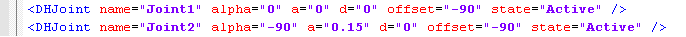
\includegraphics[scale= 0.65]{source/DHParameters.png}
  \caption{Example of configuration by DH parameters}
  \label{fig:DHParameters}
\end{figure}




